\documentclass[a4paper,12pt,fleqn,oneside]{article}
\usepackage{graphicx}
\usepackage{etex}
\usepackage[latin1]{inputenc}
\usepackage[ngerman]{babel}
\usepackage{ae,aecompl}
\usepackage[T1]{fontenc}
\usepackage{ngerman}
%\usepackage{fleqn}
\usepackage{ulem}
\usepackage{amssymb}
\usepackage[locale=DE, per-mode=fraction, quotient-mode=fraction, group-minimum-digits=6]{siunitx}
\usepackage{tabularx}
\usepackage{bm}
\usepackage{booktabs}
\usepackage{color}
\usepackage{pictex}
\usepackage[left=2.5cm,right=2.5cm,top=2cm,bottom=2cm,includeheadfoot]{geometry}
\usepackage[section]{placeins}
\usepackage{xspace}
\usepackage{multirow}
\usepackage{lastpage}
\usepackage{fancyhdr}
\usepackage{graphicx}
\usepackage{esvect}
\usepackage{pgfplots}
\usepackage[ngerman]{babel}
\usepackage{graphics}
\usepackage{graphicx}
\usepackage{tikz}
\usepackage{amsmath}
%\usepackage{autonum}
\usepackage[hidelinks]{hyperref}


\setlength{\headheight}{15pt}
\pagestyle{fancy}
\fancyfoot[C]{Seite \thepage{} von \pageref{LastPage}}
\linespread{1.5}
\author{Dominik Eisele}
\title{Laborbericht}
\date{\today}


%\begingroup\makeatletter\ifx\SetFigFontNFSS\undefined%
%\gdef\SetFigFontNFSS#1#2#3#4#5{%
%  \reset@font\fontsize{#1}{#2pt}%
%  \fontfamily{#3}\fontseries{#4}\fontshape{#5}%
%  \selectfont}%
%\fi\endgroup%


% Zusätzliche Spalten mit variabler Breite fur tabularx
%\newcolumntype{L}{>{\raggedright\arraybackslash}X} % linksbündig
%\newcolumntype{C}{>{\centering\arraybackslash}X} % zentriert
%\newcolumntype{R}{>{\raggedleft\arraybackslash}X} % rechtsbündig


\newcolumntype{L}[1]{>{\raggedright\arraybackslash}p{#1}} % linksbündig mit Breitenangabe
\newcolumntype{C}[1]{>{\centering\arraybackslash}p{#1}} % zentriert mit Breitenangabe
\newcolumntype{R}[1]{>{\raggedleft\arraybackslash}p{#1}} % rechtsbündig mit Breitenangabe


\setlength{\tabcolsep}{0pt}
\renewcommand{\arraystretch}{1}


%\renewcommand*\contentsname{Gliederung}


\let\oldsqrt\sqrt
\def\sqrt{\mathpalette\DHLhksqrt}
\def\DHLhksqrt#1#2{\setbox0=\hbox{$#1\oldsqrt{#2\,}$}\dimen0=\ht0
\advance\dimen0-0.3\ht0
%0.3 ist das Maß für die Hakenlänge, relativ zum Inhalt der Wurzel
\setbox2=\hbox{\vrule height\ht0 depth -\dimen0}%
{\box0\lower0.4pt\box2}}



\begin{document}

\begin{titlepage}
	\begin{flushleft}
		\vspace*{2\baselineskip}
		{\fontsize{16}{19.2}\selectfont Laborbericht Physik TGE12/2 A}\\[4\baselineskip]
		\begin{tabularx}{\textwidth}{rp{5px}X}
			{\fontsize{16}{19.2}\selectfont Titel:}&&{\fontsize{16}{19.2}\selectfont Millikan Versuch}
		\end{tabularx}
		\\[5\baselineskip]
		\setlength{\tabcolsep}{0pt}
		\renewcommand{\arraystretch}{1,25}
		\begin{tabular}{lp{5px}l}
			{\fontsize{14}{16.8}\selectfont Bearbeiter:}&&{\fontsize{14}{16.8}\selectfont Dominik Eisele{}}\\
			{\fontsize{14}{16.8}\selectfont Mitarbeiter:}&&{\fontsize{14}{16.8}\selectfont}\\
			{\fontsize{14}{16.8}\selectfont Datum Versuchsdurchführung:}&&{\fontsize{14}{16.8}\selectfont 11.04.2016}\\
			{\fontsize{14}{16.8}\selectfont Datum Abgabe:}&&{\fontsize{14}{16.8}\selectfont 20.06.2016}
		\end{tabular}
		\\[2\baselineskip]
		{\fontsize{14}{16.8}\selectfont Ich erkläre an Eides statt, den vorliegenden Laborbericht selbst angefertigt zu haben. Alle fremden Quellen wurden in diesem Laborbericht benannt.}
		\\[2\baselineskip]
		{\fontsize{14}{16.8}\selectfont Hochdorf, \today $  $ Dominik Eisele}
	\end{flushleft}
\end{titlepage}

\setlength{\tabcolsep}{7pt}
\renewcommand{\arraystretch}{1,7}

\newpage
\tableofcontents
\newpage


\section{Einführung}
	Der Millikan Versuch wurde erstmals im Jahr 1910 von den beiden amerikanischen Physikern Robert Andrews Millikan und Harvey
	Fletcher durchgeführt. Dabei gelang es den beiden Physikern die Elementarladung $e$ auf $e = \SI{1.592e-19}{\coulomb}$ zu
	bestimmen. Für diesen Versuch erhielt Millikan 1923 den Nobelpreis für Physik.\\
	Der heutzutage gemessene Wert beträgt $e = \SI{1.6021766208e-19}{\coulomb}$. Dieser Wert wird von der CODATA
	(Committee on Data for Science and Technology) empfohlen, bestimmt wurde er mit Hilfe des Quanten-Hall-Effekts.

\subsection{Formeln}
	Schweben mit Elektrischem Feld:
	\begin{align*}
		\left|F_{EL}\right| &= \left|F_{G}\right|\\
		q \cdot E &= m \cdot g
	\end{align*}
	Fallen ohne Elektrisches Feld:
	\begin{align*}
		\left|F_{R0}\right| &= \left|F_{G}\right|\\
		6\pi \cdot \eta \cdot r \cdot v_{0} &= m \cdot g
	\end{align*}
	Daraus Folgt:
	\begin{align*}
		q = \frac{9 \sqrt{2} \pi d}{U} \sqrt{\frac{2 \eta^3 v_0^3}{\left(\rho_{"Ol} \right) g}}
	\end{align*}
	

\newpage
\section{Material und Methoden}

\subsection{Material} 
	Der Versuch wurde mit Hilfe des Java-Applets von Carsten Groß durchgeführt. Dieses ist unter der Internetadresse
	\url{http://ne.lo-net2.de/selbstlernmaterial/p/e/mi/java1/mi_java1.html} zu finden.

\subsection{Aufbau}
	Der Aufbau des Versuchs ist in Abbilung \ref{fig:applet} zu sehen. Links ist der Ausschnitt eines Mikroskopes zu sehen, der von
	gleichmäßig angeordneten Skalenstrichen durchzogen ist. Diese Skalenstriche dienen zur Messung der Strecke die die Tröpfchen
	zurücklegen und sind in einer Entfernung von jeweils \SI{5.333e-5}{\meter} angeordnet. Daraus kann man mit dem rechts davon
	angebrachten Timer die Geschwindigkeit eines Teilchens bestimmen. Diesen Timer kann man durch unterschiedliche Methoden
	starten. Die erste Variante ist das manuelle Drücken eines Buttons, die zweite Variante ist der Start bei Polaritätswechsel und die
	dritte Variante ist der Start beim Spannungsabschalten. Die zu beobachtenten Öltröpfchen, mit einer zufälligen Elementarladung,
	kann man über den Button "`Pumpe"', von unten, in den Mikroskopausschnitt einbringen. Über den Spannungswahlregler kann
	man nun der, nach oben wirkenden Schwerkraft, entgegen wirken. Die gewählte Spannung liegt an zwei Kondensatorplatten an
	(nicht sichtbar im Java-Applet), die parallel zu den Skalenstrichen, auserhalb des Mikroskopausschnittes platziert sind.
	
	\begin{figure}[h!]
		\centering
		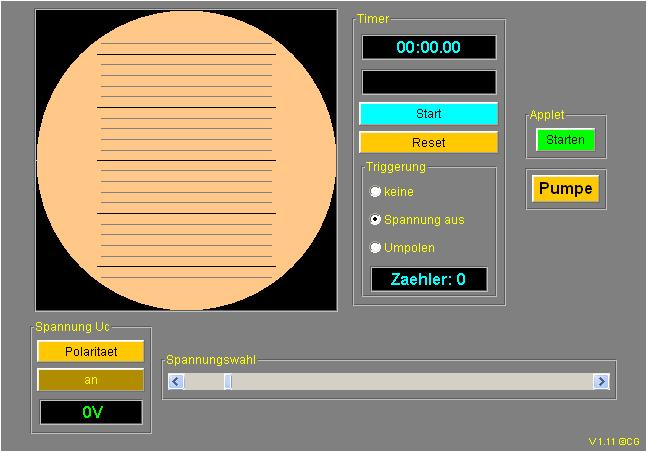
\includegraphics[width=\linewidth]{applet.jpeg}
		\caption{Versuchsaufbau}
		\label{fig:applet}
	\end{figure}

\newpage
\subsection{Durchführung}
	Über den Button "`Pumpe"' wurden Öltröpchen in den unteren Bereich des Ausschnittes des Mikroskops gegeben. Anschließend
	wurde die Triggerung auf "`Spannung aus"' gestellt, und ein Öltröpchen wurde auf einem Skalenstrich in der Schwebe gehalten.
	Dann wurde die Spannung $U_{C}$ abgeschalten, sodass dass Öltröpchen ausschließlich die Kraft $F_{G}$ erfährt. Nachdem das
	Tröpchen nun Anzahl $n$ Skalenstriche passiert hat wurde die Zeitmessung gestopt. Über diese beide Werte kann nun mit der
	Formel $v_{0} = \frac{n \cdot \SI{5.333e-5}{\meter}}{t}$ die Geschwindigkeit $v_{0}$ berechnen. Setzt man die Geschwindigkeit
	$v_{0}$ und die Spannung $U_{C}$ nun in die Gleichung $q = \frac{9 \sqrt{2} \pi d}{U} \sqrt{\frac{2 \eta^3 v_0^3}{\left(\rho_{"Ol} \right) g}}$
	ein, so erhält man die Ladung $q$ des Öltröpchens.
	
\subsection{Herleitung der Formel für die Ladung}
	\begin{align}
		q \cdot E &= m \cdot g \label{eq:1}\\
		6\pi \cdot \eta r v_{0} &= m \cdot g \label{eq:2} 
	\end{align}	
	In \eqref{eq:1} $m$ mit $m = P_{"Ol} \cdot \frac{4}{3} \pi r^{3}$ und $E$ mit $E = \frac{U}{d}$ ersetzen und nach $q$ auflösen:
	\begin{align}
		q \cdot \frac{U}{d} &= P_{"Ol} \cdot \frac{4}{3} \pi r^{3} \label{eq:3} \\
		q &=\frac{P_{"Ol} \cdot \frac{4}{3} \pi r^{3} d}{U} \label{eq:4} 
	\end{align}
	In \eqref{eq:2} $m$ mit $m = P_{"Ol} \cdot \frac{4}{3} \pi r^{3}$ ersetzen und nach $r$ auflösen:
	\begin{align}
		6\pi \cdot \eta r v_{0} &= P_{"Ol} \cdot \frac{4}{3} \pi r^{3} g \label{eq:5} \\
		r &= \sqrt{\frac{8 \cdot \eta  v_{0}}{P_{"Ol} \cdot g}}  \label{eq:6}
	\end{align}
	\eqref{eq:6} in \eqref{eq:4} einsetzen und umformen:
	\begin{align}
		q &=\frac{P_{"Ol} \cdot \frac{4}{3} \pi \sqrt{\frac{8 \cdot \eta  v_{0}}{P_{"Ol} \cdot g}}^{3} d}{U} \label{eq:7}\\
		q &= \frac{9 \sqrt{2} \pi d}{U} \sqrt{\frac{2 \eta^3 v_0^3}{\left(\rho_{"Ol} \right) g}}  \label{eq:8}
	\end{align}




\newpage
\section{Messwerte}
	Die 8 Messreihen sind in Tabelle \ref{tab:messwerte} zu sehen.\\
	Dabei ist $n$ die Anzahl an übertretenen Skalensteilen, $t$ die dafür benötigte Zeit und $U$ die an den Kondensator angelegte
	Spannung.

	\begin{table}[h!]
		\centering
		\begin{tabular}{@{}llll@{}}
			\toprule
			$n$		&	$t \text{ in }\si{\second}$	& $U \text{ in } \si{\volt}$	&	\\ \midrule
			\num{5}	&	\num{2.09}				& \num{465.0}			&	\\
			\num{5}	&	\num{2.96}				& \num{280.0}			&	\\
			\num{5}	&	\num{1.99}				& \num{250.0}			&	\\
			\num{5}	&	\num{2.83}				& \num{73.0}				&	\\
			\num{5}	&	\num{2.66}				& \num{153.0}			&	\\
			\num{5}	&	\num{3.00}				& \num{90.0}				&	\\
			\num{5}	&	\num{2.50}				& \num{379.0}			&	\\
			\num{5}	&	\num{5.73}				& \num{26.0}				&	\\ \bottomrule
		\end{tabular}
		\caption{Messwerte}
		\label{tab:messwerte}
	\end{table}


\newpage
\section{Auswertung}
	\subsection{Wertetabelle}

	\begin{table}[h!]
	\centering
	\begin{tabular}{@{}lllll@{}}
		\toprule
		Weg in $m$		& $v_{0} \text{ in }\si{\meter\per\second}$	& r in $\si{\metre}$	& $F_{G} \text{ in }\si{\newton}$	& $q \text{ in }\si{\coulomb}$	\\ \midrule
		\num{2.67E-4}	& \num{12.758E-5}						& \num{6.96E-7}		& \num{1.214E-14}				& \num{1.566E-19}			\\
		\num{2.67E-4}	& \num{9.008E-5}							& \num{5.85E-7}		& \num{7.202E-15}				& \num{1.543E-19}			\\
		\num{2.67E-4}	& \num{13.399E-5}						& \num{7.14E-7}		& \num{1.307E-14}				& \num{3.136E-19}			\\
		\num{2.67E-4}	& \num{9.422E-5}							& \num{5.98E-7}		& \num{7.704E-15}				& \num{6.332E-19}			\\
		\num{2.67E-4}	& \num{10.024E-5}						& \num{6.17E-7}		& \num{8.455E-15}				& \num{3.316E-19}			\\
		\num{2.67E-4}	& \num{8.888E-5}							& \num{5.81E-7}		& \num{7.059E-15}				& \num{4.706E-19}			\\
		\num{2.67E-4}	& \num{10.666E-5}						& \num{6.37E-7}		& \num{9.279E-15}				& \num{1.469E-19}			\\
		\num{2.67E-4}	& \num{4.654E-5}							& \num{4.20E-7}		& \num{2.674E-15}				& \num{6.171E-19}			\\ \bottomrule
		\end{tabular}
	\caption{Berechnungen}
	\label{tab:berechnungen}
	\end{table}

	In Tabelle \ref{tab:berechnungen} sind die, mit Hilfe der Daten aus Tabelle \ref{tab:messwerte}, berechneten Werte. Dafür wurden
	folgende Formeln verwendet:
	\begin{align*}
		\text{Weg} &= n \cdot \SI{5.333e-5}{\meter}\\
		v_{0} &= \frac{n \cdot \SI{5.333e-5}{\meter}}{t}\\
		r &= \sqrt{\frac{9}{2} \cdot \frac{\eta \cdot n \cdot \SI{5.333e-5}{\meter}}{P_{"Ol} \cdot g}}\\
		F_{G} &= m \cdot g\\
		q &= \frac{9 \sqrt{2} \pi d}{U} \sqrt{\frac{2 \eta^3 v_0^3}{\left(\rho_{"Ol} \right) g}}
	\end{align*}

\subsection{Diagramm}
	\begin{figure}[h!]
	\begin{tikzpicture}[xscale=1.2,yscale=1.2]
		

		\definecolor{cyan}{HTML}{0000FF}
		\definecolor{pink}{HTML}{F52887}
		\definecolor{green}{HTML}{00FF00}
		\definecolor{purple}{HTML}{461B7E}
		\definecolor{taupe}{HTML}{347235}
		\definecolor{grey}{HTML}{B6B6B4}
		\definecolor{red}{HTML}{FF0000}

		
		% Gitter
		\foreach \x in {0.5,1.0,...,9} \draw[- ,grey ,thin] (\x,0) -- (\x,7);
		\foreach \y in {0.5,1.0,...,7} \draw[- ,grey ,thin] (0.1,\y) -- (9,\y);
		\foreach \x in {1.0,...,9} \draw[- ,black ,thin] (\x,0) -- (\x,7);
		\foreach \y in {1,...,7} \draw[- ,black ,thin] (0,\y) -- (9,\y);
		% Achsen
		\draw[- ,thick] (0,0) -- (9,0) node[below right] {};
		\draw[- ,thick] (0,0) -- (0,7) node[left] {};
		% Achsbeschriftung
		\foreach \x in {,1,...,9} \draw (\x,0.05) -- (\x,-0.05) node [below] {\x};
		\foreach \y in {1,...,7} \draw (0.1,\y) -- (-0.1,\y) node [left] {$\y \cdot 10^{-19}$};
		\draw (0,0) -- (0,0) node [below left] {0};
		% Funktion
		%\draw[red, samples=50, domain=1.000244714:7] plot (\x, {sqrt((2*1.37)/(sin(\x )*9.81))});
		% Funktionbeschriftung
		%\node (11) at (7 , 1.513887287) [below] {$t=\sqrt{\frac{2s}{\sin{(\alpha)}\cdot g}}$};	
		% Messpunkte
		
		% 2V		
			\node[red]  (11) at (1,1.566) {\textsf{X}};
			\node[red]  (21) at (2,1.543) {\textsf{X}};
			\node[red]  (31) at (3,3.136) {\textsf{X}};
			\node[red]  (41) at (4,6.332) {\textsf{X}};
			\node[red]  (51) at (5,3.316) {\textsf{X}};
			\node[red]  (61) at (6,4.706) {\textsf{X}};
			\node[red]  (71) at (7,1.469) {\textsf{X}};
			\node[red]  (81) at (8,6.171) {\textsf{X}};
			1,592
			
			%\draw [black] plot [smooth] coordinates {(0,6.8) (1.7,5) (2.15,3) (2.3,0) (2.1,3) (1.3,5) (0,6)};
		
	\end{tikzpicture}
	\caption{Diagramm Ladung}
	\label{fig:Diagramm}
	\end{figure}
	
	In Diagramm \ref{fig:Diagramm} sind die Ladungen der Öltröpchen eingezeichnet. Die Messwerte stehen in keinem Zusammenhang
	zueinander, ihre einzige Gemeinsamkeit ist, dass alle Ladungen ein vielfaches der Elementarladung $e$ sind.
\newpage


\section{Quellen}
	\begin{itemize}
		\item Millikan, R. A. (1911): The Isolation of an Ion, a Precision Measurement of its Charge, and the Correction of Stokes's
			 Law in: Physical Review (Series 1) Vol. 32, Issue 4, April 1911, S. 349-397 (doi:10.1103/PhysRevSeriesI.32.349),
			 eingereicht im Nov. 1910
		\item \url{http://physics.nist.gov/cgi-bin/cuu/Value?e}, abgerufen am 19.06.2016
	\end{itemize}


\end{document}
